\documentclass[12pt, a2paper, portrait]{tikzposter}
\tikzposterlatexaffectionproofoff

\usetitlestyle{Empty}
\usebackgroundstyle{Empty}
\usepackage{wrapfig}
\usepackage[utf8]{inputenc}
\usepackage{physics}
\usepackage[mathscr]{euscript}  % \mathscr
\usepackage{mhchem}
\usepackage{subcaption}
\usepackage{mathtools}

%   Define a HUGE command, for the title
\makeatletter
\newcommand\HUGE{\@setfontsize\Huge{45}{0}}
\makeatother


%
%   Improve author and affiliation design
%
\usepackage{authblk}

% Loading authblk leads to a very large vspace after the title. https://tex.stackexchange.com/a/352566/106914
\makeatletter
\renewcommand\maketitle{\AB@maketitle} % revert \maketitle to its old definition
\renewcommand\Affilfont{\Large} % set font for affiliations
\makeatother



%
%   Define colors
%
\usepackage{xcolor}
\definecolor{ugent_blue}{RGB}{30, 100, 200}
\newcommand{\textcbf}[1]{\textcolor{ugent_blue}{\textbf{#1}}}  % text colorized and bold-faced


\definecolorstyle{myColorStyle} {} {
    \colorlet{blocktitlebgcolor}{ugent_blue!80}
}
\usecolorstyle{myColorStyle}

\bibliographystyle{unsrt}



%
%   TITLE
%

\title{
    \parbox{\linewidth}{ \center
        \HUGE{
            \textcolor{ugent_blue}{
                \textbf{
                    A chemical explanation of graph neural networks
                }
            }
        }
    }
}

\renewcommand\emph[1]{\textcolor{ugent_blue}{\textbf{#1}}}
\renewcommand\refname{\vskip -1cm}
\renewcommand{\familydefault}{\sfdefault}  % for the main font, use sans serif Computer Modern



%
%   AUTHORS AND AFFILIATIONS
%
\author[$\dagger$]{X. Wieme} 
\author[$\dagger$]{A. Gevaert} 
\author[$\dagger$]{Y. Saeys}


\affil[$\dagger$]{Ghent University, Krijgslaan 281 (S3), B-9000 Gent, België}

%
%   MAIN DOCUMENT
%

\begin{document}

\maketitle

\begin{columns}
	% Left Column.
	\column{0.5}
	% Introduction block.
    \block[titleinnersep=0.3cm, bodyinnersep=0.5cm, linewidth=0.15cm]{Introduction} {
		% This block should always be there and should briefly introduce your research. Citations can be made as normal \cite{acke2020a}. If you want to \emph{emphasize} something, you can.

		\begin{itemize}

			\item \emph{Opaque predictions} for machine learning models builds \emph{trust issues} and restricts creation of
			      novel scientific insights found by those models.\cite{carvalho2019machine}.

			\item Current explainable artificial intelligence techniques \emph{fail} to provide a \emph{chemically intuitive
				      explanation}.\cite{yuan2022explainability}

			\item Recently, Wu et. al. developed a chemically intuitive explanation technique for graph
			      neural networks by assigning attributions to \emph{chemical substructure} (e.g. functional groups,
			      BRICS, MURCKO).\cite{wu2023chemistry}

			\item The difference between the model prediction of a molecule and a masked molecule is a
			      too simple attribution. A popular method to distribute the model prediction over the
			      features is the \emph{Shapley value}.\cite{molnar2020interpretable} However, the Shapley value does not take the graphical
                  structure into account. Therefore, the Hamiache-Navarro value \cite{hamiache_value_1999}, which extends the Shaple 
                  value to graphs, will be compared with the Shapley value.

		\end{itemize}

	}

	\block[titleinnersep=0.3cm, bodyinnersep=0.5cm, linewidth=0.15cm]{Explain graph neural networks using the Shapley and Hamiache-Navarro value}{

        Players can be determined based on functional groups (left) or BRICS bonds (right).

		\begin{tikzfigure}
			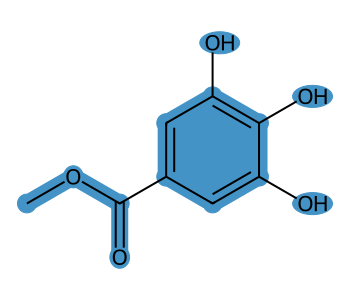
\includegraphics[scale=0.7]{../data/images/example_functional_groups.png}
			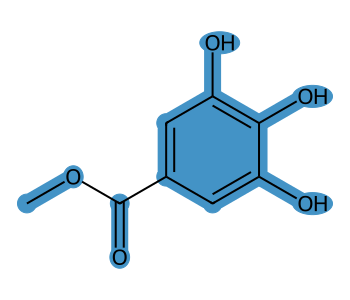
\includegraphics[scale=0.7]{../data/images/example_brics.png}
		\end{tikzfigure}
	}

    
	% Block containing the references.
	\block[titleinnersep=0.3cm, bodyinnersep=0.8cm, linewidth=0.15cm]{References} {
		\vspace{-0.5cm}
		\bibliography{poster.bib}
	}

	\column{0.5}
	% Theory
	\block[titleinnersep=0.3cm, bodyinnersep=0.5cm, linewidth=0.15cm]{Theory}{
		% Add a small theory section. Keep your theory short and to the point.
		\section{Shapley value}

		Let $(N, v)$ be a game with a set of players $N$ and a characteristic function
		satisfying $2^N \coloneqq \{S | S \subseteq N\} \rightarrow \mathcal{R}, \; v(\emptyset) = 0$.
		The Shapley value $\phi_i$ of player $i$ is defined as\cite{shapley1953value}

		\begin{equation}
			\phi_i = \sum_{S \subseteq N \ \{i\}} \frac{\left( |N| - 1 - |S| \right)! |S|!}{|N|!} \left(v(S \cup \{i\}) - v(S) \right)
		\end{equation}

		\section{Hamiache-Navarro value}

		Let $(N, v, g)$ be a game with communication structure given by the graph $\left< N, g \right>$, where
		$g \subseteq g_N \coloneqq \{ \{i, j\} | i, j \in N \}$ is the set of adjacent players. The
		associated game $(N, v^*, g)$ is defined as

		\begin{equation}
			v^*(S) =
			\begin{cases}
				v(S) + \tau \sum_{j \in \mathcal{N}(S)} \left[ v(S \cup \{j\}) - v(S) - v(\{j\}) \right] & \text{if } |S/g| = 1 \\
				\sum_{R \in S/g} v^*(R)                                                                  & \text{otherwise}
			\end{cases}
			.
		\end{equation}
	}

    \block[titleinnersep=0.3cm, bodyinnersep=0.5cm, linewidth=0.15cm]{Relational graph neural network}{

    }


	% Contact and Acknowledgements block.
	\block[titleinnersep=0.3cm, bodyinnersep=0.5cm, linewidth=0.15cm]{Contact and acknowledgements} {
		Contact via email at xander.wieme@ugent.be. \\
		\begin{wrapfigure}[1]{r}{10cm}
			\vspace{-2.7cm}
			\begin{tikzfigure}[]
				
\includegraphics[height=2cm]{figures/ugent_logo}
			\end{tikzfigure}
		\end{wrapfigure}
	}


\end{columns}

\end{document}
